\documentclass[a4paper,11pt]{article}

%--------------------------------------------------------------------------
% Pacotes Necessários
%--------------------------------------------------------------------------
\usepackage[brazil]{babel} % padronizar a linguagem
\usepackage[utf8]{inputenc} % permitir a acentuação
\usepackage[protrusion=true,expansion=true]{microtype} % obter melhor tipografia
\usepackage[svgnames]{xcolor} % habitar cores para 'svgnames'
\usepackage[hang, small,labelfont=bf,up,textfont=it,up]{caption} % customizar captions acima/abaixo de tabelas ou figuras
\usepackage{color}    % definir cores
\usepackage{graphicx} % adicionar imagens
\usepackage{fix-cm}   % customizar o tamanho das fontes
\usepackage{sectsty}  % habilitar a customização dos títulos das seções
\usepackage{fancyhdr} % definir cabeçalhos e rodapés
\usepackage{listings} % listagens
\usepackage[ddmmyyyy]{datetime} % mostrar a data
\usepackage{titling} % Permite a configuração do título
\usepackage{url} % codigo para as URLs
\usepackage{enumitem} % Configurar as Listas
\usepackage[a4paper, inner=1.5cm, outer=3cm, top=2cm, bottom=3cm, 
bindingoffset=1cm]{geometry}
%--------------------------------------------------------------------------
% Definições Iniciais
%--------------------------------------------------------------------------

% modificar toda a fonte de todas as seções
\allsectionsfont{\usefont{OT1}{phv}{b}{n}}
% habilitar a customização de cabeçalhos e rodapés
\pagestyle{fancy} 

\addto\captionsenglish{ % modificar os nomes do ingles
	\renewcommand{\abstractname}{Resumo}
	\renewcommand{\bibname}{Consulte também...}
	\renewcommand{\contentsname}{Sumário}
	\renewcommand{\listfigurename}{Figuras}
	\renewcommand{\lstlistingname}{Listagem}
	\renewcommand{\lstlistlistingname}{Listagens}
	\renewcommand{\refname}{Referências}
}

\definecolor{codegray}{rgb}{0.5,0.5,0.5}
\definecolor{backcolour}{rgb}{0.95,0.95,0.92}

% Definição para as caixas de listagens
\lstset {
	aboveskip=3mm,
	backgroundcolor=\color{backcolour},
	basicstyle={\small\ttfamily},
	belowskip=3mm,
	breaklines=true,
	breakatwhitespace=true,
	columns=flexible,
	commentstyle=\textit,
	frame=tb,
	keepspaces=true,
	keywordstyle=\color{blue}\bfseries,
	% language=Java, Python, HTML, CSS
	numbers=left,
	numbersep=5pt,
	numberstyle=\tiny\color{codegray},
	showstringspaces=false,
	showtabs=false,
	tabsize=3
}

% Cabeçalhos - limpar tudo
\lhead{}
\chead{}
\rhead{}

% Rodapés
\lfoot{\tiny Docker}
\cfoot{\tiny Versão 2.0}
\rfoot{\tiny Folha \thepage\ }

\title{Roteiro Palestra Docker}
\author{
  Fernando Anselmo \\
  \texttt{fernando.anselmo74@gmail.com} \\
}

\begin{document}
\maketitle

\section*{Comandos Iniciais}
{\ttfamily\$ docker version} \\
{\ttfamily\$ docker images} \\
{\ttfamily\$ docker ps -a}

\section{Caso MySQL}
MySQL é um sistema de gerenciamento de banco de dados, que utiliza a linguagem SQL. Atualmente é um dos SGBD mais populares. \\
{\ttfamily\$ docker pull mysql} \\
{\ttfamily\$ docker run --name mybanco -e MYSQL\_ROOT\_PASSWORD=root -p 3306:3306 -d mysql} \\[2mm]
Nas próximas vezes: \\
{\ttfamily\$ docker start mybanco} \\
{\ttfamily\$ docker exec -it mybanco sh -c 'exec mysql -u root -p'} \\
{\ttfamily\$ docker exec -it mybanco bash} \\
{\ttfamily root@b38dfbb9c50d:/\# mysql -u root -p} \\
{\ttfamily mysql> select @@version;} \\
{\ttfamily\$ docker stop mybanco}

\section{Caso Pentaho}
Pentaho é um software de código aberto para inteligência empresarial, desenvolvido em Java. A solução cobre as àreas de ETL, reporting, OLAP e mineração de dados. \\
{\ttfamily\$ docker pull wmarinho/pentaho} \\
{\ttfamily\$ docker run --name pentaho-server -p 8080:8080 -d wmarinho/pentaho} \\[2mm]
Acessar a imagem: \\
{\ttfamily\$ docker exec -it pentaho-server bash} \\[2mm]
Podemos ver aonde está o Pentaho: \\
{\ttfamily\# echo \$PENTAHO\_HOME} \\[2mm]
Ou podemos acessá-lo pelo navegador no endereço: \url{http://localhost:8080/pentaho/Login}. Usuário: admin. Senha: password.

\section{Caso PostgreSQL}
PostgreSQL é um sistema de gerenciamento de banco de dados relacional de objetos (ORDBMS) com ênfase em extensibilidade e conformidade com padrões. Lida com cargas de trabalho que variam de pequenos aplicativos a grandes aplicativos voltados para a Internet (ou para armazenamento de dados) com muitos usuários simultâneos. \\
{\ttfamily\$ docker pull postgres} \\
{\ttfamily\$ docker run --name postbanco -e POSTGRES\_PASSWORD=postgres -d -p 5432:5432 \\ postgres} \\
{\ttfamily\$ docker start postbanco} \\
{\ttfamily\$ docker stop postbanco}

\section*{Docker Compose}
Compose é uma ferramenta para definir e executar aplicativos Docker com vários contêineres. \\
{\ttfamily\$ docker-compose build} \\
{\ttfamily\$ docker-compose rm} \\
{\ttfamily\$ docker-compose (up | down)} \\
{\ttfamily\$ docker-compose (start | stop)} \\
{\ttfamily\$ docker-compose run -d} \\
{\ttfamily\$ docker-compose exec} \\
{\ttfamily\$ docker-compose logs (-f)}

\section{Caso PostgreSQL Compose}
Arquivo: docker-compose.yml
\begin{lstlisting}
version: '2'
services:
db:
 image: postgres
  restart: always
  environment:
   POSTGRES_PASSWORD: postgres
   POSTGRES_USER: postgres
  ports:
   - 5432:5432
  adminer:
   image: adminer
   restart: always
   ports:
    - 8080:8080
  client:
   image: postgres
   depends_on:
    - db
   command: psql -U postgres --password -h db
  db-legacy:
   image: postgres:9.5
   restart: always
   environment:
    POSTGRES_PASSWORD: postgres
    POSTGRES_USER: postgres
   ports:
    - 5532:5432
\end{lstlisting}
Levantar os contêineres: \\
{\ttfamily\$ docker-compose up} \\[2mm]
Nova aba do terminal na mesma pasta: Ctrl + Shift + T
{\ttfamily\$ docker-compose ps} \\
{\ttfamily\$ docker-compose run client} \\
{\ttfamily\# create database teste;} \\
{\ttfamily\# \textbackslash connect teste;} \\
{\ttfamily\# create table base(id serial not null, nome varchar(50), primary key (id));} \\
{\ttfamily\# \textbackslash d} \\
{\ttfamily\# \textbackslash dS+} \\
{\ttfamily\# \textbackslash d base} \\
{\ttfamily\# \textbackslash q} \\
{\ttfamily\$ docker exec -it palestra\_db-legacy\_1 psql -U postgres --password} \\[2mm]
Encerrar: \\
{\ttfamily\$ docker-compose down}

\section{Caso NGINX}
Nginx é um servidor web rápido, leve, e com inúmeras possibilidades de configuração para melhor performance. Criar a seguinte estrutura de arquivos:
\begin{figure}[!htb]
	\centering
	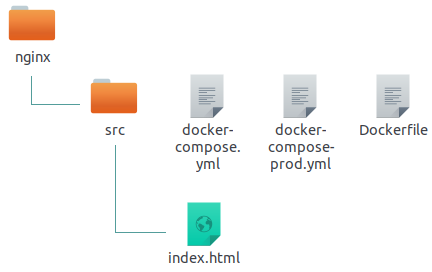
\includegraphics[width=0.6\textwidth]{imagem/estnginx.png}
	\caption{Estrutura dos Arquivos}
\end{figure} \\
1. Arquivo "src/index.html"
\begin{lstlisting}
<html>
 <body>
  <h1>Hello World</h1>
 </body>
</html>
\end{lstlisting}
2. Arquivo "Dockerfile"
\begin{lstlisting}
FROM nginx
COPY src /usr/share/nginx/html
\end{lstlisting}
3. Arquivo "docker-compose.yml"
\begin{lstlisting}
version: '2'
services:
 app:
  build: .
  image: app:1.0.0
  volumes:
   - ./src:/usr/share/nginx/html
  ports:
   - 8080:80 
\end{lstlisting}
4. Arquivo "docker-compose-prod.yml"
\begin{lstlisting}
version: '2'
services:
 app:
  build: .
  image: app:1.0.0
  ports:
   - 80:80 
\end{lstlisting}
As ações serão as seguintes: \\
{\ttfamily\$ docker-compose up --build} \\
Acessar \url{http://localhost:8080} \\
Acessar outro terminal [CTRL+SHIFT+T] \\
{\ttfamily\$ docker-compose down} \\
{\ttfamily\$ docker-compose -f docker-compose-prod.yml up --build} \\
Acessar \url{http://localhost} \\
{\ttfamily\$ docker-compose down}

\section{Caso DJango}
Django é um framework para desenvolvimento rápido para web, escrito em Python, que utiliza o padrão model-template-view. Exemplo em: \url{https://gist.github.com/shudarshon/cf56741e6bcc26bedd4db236447e1654}: \\
{\ttfamily\$ docker-compose build} \\
{\ttfamily\$ docker-compose up -d} \\
{\ttfamily\$ docker-compose logs} \\
{\ttfamily\$ docker inspect exdjango\_postgres\_1 | grep IP}
{\ttfamily\$ psql -h 172.17.0.3 -p 5432 -U postgres --password}
{\ttfamily\$ docker-compose down}

\section{Caso Raspberry Pi}
Necessidades:
\begin{itemize}[noitemsep]
	\item Cabo crossover
	\item Fonte alimentação Raspberry (cabo mini USB)
\end{itemize}
Descobrir o Raspberry na rede:
\begin{enumerate}
	\item Qual o prefixo do seu IP da Rede (na qual deve estar o Raspberry)? \\ {\ttfamily\$ ifconfig}
	\item Localizar o Raspberry no mesmo prefixo de IP (p.e. 192.168.10.x) \\ {\ttfamily\$ nmap -n -sP 192.168.10.255/24} (daqui para frente assumirei o IP do Raspberry como 192.168.10.2)
\end{enumerate}

\subsection{Instalar a Docker Machine}
{\ttfamily\$ base=https://github.com/docker/machine/releases/download/v0.14.0 \&\&
curl -L \$ base/docker-machine-\$(uname -s)-\$(uname -m) > /tmp/docker-machine \&\& sudo install /tmp/docker-machine /usr/local/bin/docker-machine} \\[2mm]
Para copiar arquivo para o Raspberry: \\
{\ttfamily\$ scp machine.png pi@192.168.25.2:/home/pi/html} \\[2mm]
Tabela de Roteamento IP do Kernel \\
{\ttfamily\$ netstat -rn} \\[2mm]
Acessar o Raspberry: \\
{\ttfamily\$ ssh pi@192.168.10.2} (Senha: \textbf{raspberry}) \\
{\ttfamily\$ sudo nano /etc/os-release} \\
Mudar o id: \textbf{ID=raspbian} para \textbf{ID=debian} \\
{\ttfamily\$ curl -sSL https://get.docker.com | sh} \\
{\ttfamily\$ sudo usermod -aG docker pi} \\
{\ttfamily\$ exit}

\subsection{Gerar as chaves: particular e pública}
{\ttfamily\$ ssh-keygen -b 2048 -t rsa (key:id\_rsa passphrase:raspberry)} \\
{\ttfamily\$ cat ~/.ssh/id\_rsa.pub | ssh -p 22 pi@192.168.10.2 'cat >>.ssh/authorized\_keys'}

\subsection{Instalar o Docker no Raspberry}
Comandos no Raspberry: \\
{\ttfamily\$ nano /etc/ssh/sshd\_config} \\
Parâmetro: '\textbf{\#PasswordAuthentication yes}' para '\textbf{PasswordAuthentication no}' \\
{\ttfamily\$ sudo /etc/init.d/ssh restart}

\subsection{Criar a Docker Machine}
{\ttfamily\$ docker-machine create --driver generic --generic-ip-address 192.168.10.2 \\ --generic-ssh-key ~/.ssh/id\_rsa --generic-ssh-user pi --engine-storage-driver \\ overlay2 pi-zero-1} \\
{\ttfamily\$ docker-machine ip pi-zero-1}

\subsection{Após Criada a Docker Machine}
{\ttfamily\$ docker-machine env pi-zero-1} \\
{\ttfamily\$ eval \&(docker-machine env pi-zero-1)} \\[2mm]
Testar: \\
{\ttfamily\$ docker-machine ssh pi-zero-1} \\[2mm]
Criar uma pasta html/ e nela um arquivo index.html simples. \\
{\ttfamily\$ exit} \\
{\ttfamily\$ docker run -d -p 80:80 --name nginx2 -v /home/pi/html:/var/www/html tobi312/rpi-nginx} \\
Acessar: \url{http://192.168.10.2/}

\subsection{Finalizar}
{\ttfamily\$ ssh pi@192.168.10.2} (Senha: raspberry) \\
{\ttfamily\$ sudo halt}
\end{document}